\documentclass[12pt]{article}

% \usepackage[utf8]{inputenc}
% \usepackage[T1]{fontenc}
% \usepackage{authblk}

\usepackage[backend=biber,style=authoryear]{biblatex}
\renewcommand*{\nameyeardelim}{\addcomma\space}
%\usepackage{biblatex}

\usepackage[a4paper, top=3cm, left=3cm, bottom=2cm, right=2cm]{geometry}
\usepackage{indentfirst}
\setlength{\parindent}{1.25cm}

% \usepackage[no-math]{fontspec}
% \defaultfontfeatures{Ligatures=TeX}
% \setmainfont{Tex Gyre Termes}

\usepackage{lmodern} % Latin Modern Font

\usepackage[nodisplayskipstretch]{setspace}
\setstretch{1.427465}

\usepackage[explicit]{titlesec}
\titleformat{\section}[hang]{\normalfont\bfseries}{\thesection}{1em}{\MakeUppercase{#1}}
\titleformat{\subsection}[hang]{\normalfont}{\thesubsection}{1em}{\MakeUppercase{#1}}
\titleformat{\subsubsection}[hang]{\normalfont\bfseries}{\thesubsubsection}{1em}{#1}%{\MakeLowercase{#1}}
\newcommand{\sectionbreak}{\clearpage}

\usepackage{titletoc}
\titlecontents{section}[1em]{\vspace{12pt}}{\bfseries\normalsize\contentslabel[\thecontentslabel]{3em}\uppercase}{\hspace*{-2em}\uppercase}{\titlerule*[.75em]{.}\contentspage}
\titlecontents{subsection}[1em]{\vspace{12pt}}{\normalfont\normalsize\contentslabel[\thecontentslabel]{3em}\uppercase}{\hspace*{-2em}\uppercase}{\titlerule*[.75em]{.}\contentspage}
\titlecontents{subsubsection}[1em]{\vspace{12pt}}{\bfseries\normalsize\contentslabel[\thecontentslabel]{3em}}{\hspace*{-2em}}{\titlerule*[.75em]{.}\contentspage}


\usepackage{amsmath}  % enables declare math operator
\DeclareMathOperator{\sign}{sign}

\usepackage{amsfonts} % \mathbb
\usepackage{graphicx} % manipulate imported images


\usepackage{fancyhdr} % \pagestyle{fancy}
\fancyhf{}
\fancyhead[R]{\thepage}
\renewcommand{\headrulewidth}{0pt}

\usepackage[toc, section=section]{glossaries}
\makeglossaries

\usepackage{hyperref}
\usepackage{hypcap}
\hypersetup{
  colorlinks=true, 
  allcolors=black,
  pdfauthor={Carlos Henrique Tarjano Santos},
  pdftitle={Robust Digital Envelope Estimation Via Geometric Properties of an Arbitrary Real Signal}
}

\bibliography{Envelope,Compression}
  
\title{Sound Synthesis}
\author{Carlos Henrique Tarjano Santos}

\newacronym{FPS}{FPS}{frames per second}
\newacronym{LMS}{LMS}{Least Mean Squares}

% \newglossaryentry{VST}{name=VST, description={Virtual Studio Technology}}



\begin{document}

%\documentclass[12pt]{article}
\usepackage[a4paper, top=3cm, left=3cm, bottom=2cm, right=2cm]{geometry}
\usepackage[utf8]{inputenc}
% \usepackage{fontspec}
% \setmainfont{Arial}
\title{Sound Synthesis}
\author{Carlos Tarjano}
\usepackage[portuguese]{babel}

\begin{document}


\begin{abstract}

\end{abstract}

{\bf Palavras-chave:}


\end{document}

\pagestyle{empty}

\begin{abstract} % 150 words

\end{abstract}

{\bf Keywords:}

% \newpage
% \listoffigures % lista de ilustracoes

% \newpage
% \listoftables % lista de tabelas

\newpage
\tableofcontents

\newpage
\pagestyle{fancy}

\newacronym{ENIAC}{ENIAC}{Electronic Numeric Integrator and Calculator}

\section{Introduction}
% Tell the reader the problem you are tackling in this project.
The area of artificial intelligence and, more specifically, neural networks, is interdisciplinar since its conception, being born from biological inspirations. Implementation wise, connections with fields like programming, computing and mathematics imposed themselves since the begining.

Attention, however, seems to revolver around the use of advancements in related disciplines to the betterment of neural networks theory in general, be it in the form of convolutional networks, better hyperparameter search, parallel implementations, etc.
Generally, neural networks are applyied to some problem, with little concern about transforming the problem in order to make it optimally suited to work in a neural networks approach, outside of necessary adaptations, such as normalization.

This lack is in part justified by the recent progress exhibted in the field, where impressive results are abundant; a word of caution is needed here, however, as this is a field that experimented its fair share of hype cycles, followed by winters.
neural networks faced many winters since its introduction. The pattern seems to repeat itself: hardware improvements enable attractive new results, the interest rises, and some technical advancements are made. 
Although, in its current renaissance, the field is still blooming, there are some that are already pointing to a decrease in the research output.

We feel that this tool still offers a great potential in its current state of development; a potential thtat will only be fully explored once it is realised that workflows and auxiliary theories are needed, to be used in conjunctions with neural networks.

In this sense, we introduce a novel representation for pseudo periodic time series, of which sound representation are our primary interest. Although much of the theory is drawn from conventional areas related to digital signal processing, image processing, etc, the representation was formulated from the beginning having in mind the strengths and limitations of neural networks in general.
% State clearly how you aim to deal with this problem. 

In this context, the primary objective of this work is to illustrate how such integration can be done, by developing a new sound representation designed specifically to be used by neural networks in sound synthesis tasks.

Since the beginning of computing, even when mainframes were the only available medium, restricted to organizations with considerable budgets, people found ways and motivation to overcome the technical limitations and develop artistic applications, like video games, in their (and the machine's) spare time. 


On a parallel note, also relevant to this thesis, those first machines, like the \gls{ENIAC} in 1946, brought with then the promise of the artificial intelligence as their ultimate goal \parencite{2010DonovanReplay}.

Music, on the other hand, is another staple of humanity's creativity. % TODO first musical instruments
 Is only natural that, as soon as this technology became reasonably stable, musical applications started to emerge.

Ambitious as it may seem, it is the goal of this monograph to motivate a change of approach in domains that, despite their modest intersections, share more attributes than is apparent at a superficial glance: Both machine learning and digital musical acoustics are areas that, despite their current relevance, are fresh out of their respective infancies, and a scrutiny of both promptly reveals the difficulties that arise from this state of affairs. A lack of their own terminology, with frequent borrows from other, more established areas, can be readily cited, as the pronounced prominence of few individual contributions.

Those shortcomings have, however, a bright side to them, in that they still expose those areas to reinterpretation, rendering them somewhat open to the influence of outside ideas.

Digital musical acoustics borrows heavily from the digital signal processing terminology, the last having its roots in the analogic world. Many algorithms are conceived in terms of filters, circuits and other similar legacy constructs, a fact that burdens the conceptual, theoretical framework of the area. Besides the introduction of a noveau envelope extraction method, we find that his formulation in terms of (differential) geometric concepts is, perhaps, as great a contribution as the algorithm per se.

% Limit the scope of your study. 

% Sketch out how the thesis is structured to achieve your aim. 


% objective


\section{Bibliographic Approach}

With the advance of technology, some classic problems of bibliographic research were mitigated, while new ones were introduced. Fe
w would argue that the ability to carry thousands of books in a handheld device wasn't an improvement, with accessibility improvements such as the possibility of hearing text, instead of reading it, distribution, etc revolutionizing the consumption, creation of knoledge. This revolution was not without its drawbacks, however.

A modern problem encountered by the author during the development of this work is the fragmentation of data. In the bygone days of physical research, a paper existed, in the researcher files, in one physical location. All the metadata available, perhaps even notes, where in a single logic object, such as a book or a photocopy. 

When access to the original document was limited, such as a piece of literature residing in a library, nevertheless the approach could be the same, the logical object now being a card sumarizing the metadata and relevant content. This approach is, of course, translatable to the digital world, where one could maintain a folder where digital files, such as pdfs, reside, with notes and the relevant metadata embedded in the file, its filename of even in the metadata section.

This approach quickly becomes problematic, however, for scientific writting, specially in the context of bigger productions such as books and, as is the present case, a thesis, for a number of reasons. Digital documents, especially the most common ones, are designed to be as generic as possible, serving variated purposes, as are their metadata systems, if present.

The management of metadata is best acomplished with the used of dedicated software, of which zotero and mendeley are some examples, Being specifically designed to this task, facilities such as metadata retrieval and validation are often available. If on intends to make use of a typesetting system, such as Latex, avoiding bibliographic management software is virtually impossible.

Another problem in bibliography management in the digital era is to maintain syncronized the original files, most commonly available in pdf or epub format, and generally trated as general files by most file brownsing interfaces, and its metadata, that must exhib a more sophisticated and uniform structure.
pdf, despite its ubiquity, is a tricky format, being somewhat opaque. Besides, multiple ways exist to encode a similar document. Fortunately, we don't need to extract correct or even meaninful text from it, the only thing we need is a way tu uniquely identify each file, impevious to file changes such as the addition of comments, changes in location in the filesystem or renaming.

bibtex uses keys. as tempting as it might sound to use those keys as identifiers fro the files, that approach presents problems.

we adress the meta problem of organizing the bibliography introducing a piece of bibliographic software based on an novel paradigm.




writing a phd thesis is a peculiar endeavour in the academic world, in the sense that it is a requirement that must be fullfilled only once: while a thriving academic carreer pressuposes a constant output of papers, and possibly books, or book chapters, the closest contact an academic has with the format of a thesis is probably during the development of his masters dissertation; that one endeavour being, all in all, substantially different.

It comes as no surprise, then, that bibliographic software, being in general geared towards the task of aiding in the productions of academic articles, can be subpar for a thesis, where the hability to handle a mutch larger volume of bibliographic material is needed.

\section{Conventions and definitions}
The field explored in this work, besides being extensive and fragmented, is largely interdisciplinar, with terminology strong influenced by widespread usage in the community rather than academic tradition. To maintain coherence thougout the text, it is convenient to stablish some definitions, as some of the terms here applyed may deviate from their usage in particular fields.

Effort was made to comply with the most commom nomenclature when terms are encountered frequently in literature.

This work will make extensive use of the term sample, that, even in the context of digital signal processing, can be ambiguous. It can refer to a, usually short, sound file, as when refering to sample based instruments, or it can sometimes mean a unique point of a discrete sound wave, as when used in sample rate. We will adopt the first meaning, and prefer frame for the second; altough the usage is more comum when referring to videos, it is used in terms such as frames per second.

\section{Theory}

In this sections we present some topics that will serve as basis for later chapters, from a purely theoretical point of view. This is specially important in this work, since many different, seemingly disconnected areas are brought togheter.

\subsection{Waves}

It can be insightful to analyse the behaviour of the crytical points and the zeroes of an arbitrary, periodic wave over time.
We will assume, for the sake of simplicity, that each cycle of said wave has a unique maximum and minimum, and crosses the horizontal axis one single time. Those assumption dont compromise the generality of the analysis, as in the case of multiple maxima, minima and/or zeroes, one of thosee can be choosen randomly to represent the global one, as long as consistency between cycles is maintained.

We are going to also assume that a wave with a zero phase has an maximum instantaneous amplitude at time zero, as is the case of the cosine wave, for example. Altough that assumption somewhat departs from the physical intuition, it is useful in making our description consistent with the theory behind the Fourier Transform.

For a continuous wave, if we were to plot the time at which any of those values ocurred as a function of their ordinality, the result would be parallel straight lines, their slope somehow related to the frequency of the underlying wave. We will illustrated the point in the case of discrete waves, as this case will be of more immediate use in this work.

\subsubsection{Continuous and discrete waves}

First, it is necessary to establish a correspondence between a continuous and a discrete wave, as the latter will be the object of most of this work. To do that we will define a simple continuous sinusoidal wave of the form $ S(t) = a \cos \left( \phi + 2 \pi \mathcal{F} t \right) $, where $ a \in \mathbb{R}^+ $ is the amplitude; $ \phi \in \mathbb{R}^+, 0 \le \phi < 2 \pi $ is the phase; $ \mathcal{F} \in \mathbb{R}^+ $ is the absolute frequency of the wave, in Hz and $ t \in \mathbb{R} $ is time, in seconds.

The cosine function is used for a twofold reason: its use helps to underline the periodic nature of the wave in consideration and is the parameter of the phase when the FT is used. It is important to keep in mind, however, that this discussion applies any arbitrary function of the form $ f(x) = f(x + P) \forall x \in D(f) $, where $ D $ is the domain of the function $ f $.
% TODO This will be further illustrated in the discrete part below.

If we were to sample $ S(t) $ at regular intervals, that is, to measure the value of the function at a constant rate of $ h $ \gls{FPS}, neglecting errors of measurement, we would have a discrete representation of the continuous wave of the form $ W[i] = a \cos \left( \phi + 2 \pi f \frac{i}{n} \right) $ where, alongside the quantities introduced before, we would have $ i \in \mathbb{N} $ as the frame number; $ n \in \mathbb{N} $ as the number of discrete samples and $ f \in \mathbb{R}^+ $ being the relative frequency of our discrete wave in cycles per $ n $ samples.

The relative, local frequency $ f $ of the discrete representation is related to the absolute frequency $ \mathcal{F} $ via the equation $ f = \frac{n}{\text{fps}} \mathcal{F} $ while the absolute time, in the continuous case can be obtained from the frame number $ i $ of the discrete signal via $ i = t \ \text{fps} $.

\subsubsection{Points of interest of periodic waves}



\subsection{Least Mean Squares}



The linear \gls{LMS}, also known as linear regression \parencite{2018StephenBoydIntroduction} is a data fitting technique. % TODO

We present here the theory for real numbers, noting that it can be easily extended for complex numbers \parencite{1995LawsonSolving}, should the necessity arise. That, however, will not be the case in this work.

Given two vectors $ X $ and $ Y $, such that:
$$ X = [x_0, x_1, \cdots ,x_{m-1}]^T, \ x_i \ \in \ \mathbb{R} \ \forall \ i, \ 0 \le i < m \in \mathbb{N} $$
$$ Y = [y_0, y_1, \cdots ,y_{m-1}]^T, \ y_i \ \in \ \mathbb{R} \ \forall \ i, \ 0 \le i < m \in \mathbb{N} $$
We ideally want to find the vector of coefficients $ A = [a_0, a_1, \cdots ,a_k]^T, \ a_j \ \in \ \mathbb{R} \ \forall \ j, \ 0 \le j \le k \in \mathbb{N} $ that satisfies the equality $ x^0_i a_0 + x^1_i a_1 + \cdots + x^{k-1}_i a_{k-1} + x^k_i a_k = y_i \quad \forall \quad i \in \{0, \cdots , m-1\} $.

Put in that way, what we have is a system of linear equations that can be rewritten in matrix form as seen in equation \ref{eq:lms}.

\begin{equation}
  \label{eq:lms}
\stackrel{Q_{m \times (k+1)}}
{
\begin{bmatrix}
1 & x_0 & \cdots & x_0^k \\
1 & x_1 & \cdots & x_1^k \\
\vdots & \vdots & \ddots & \vdots  \\
1 & x_{m-1} & \cdots & x_{m-1} \\
\end{bmatrix}
}
\stackrel{A_{(k+1) \times 1}}
{
\begin{bmatrix}
a_0 \\
a_1 \\
\vdots  \\
a_k \\
\end{bmatrix}
}
=
\stackrel{Y_{m \times 1}}
{
\begin{bmatrix}
y_0 \\
y_1 \\
\vdots  \\
y_{m-1} \\
\end{bmatrix}
}
\end{equation}

More compactly, we have that $ Q A = Y $. This system will generally be over-determined, only having an exact solution in the case where $ Y $ is a linear combination of the columns in $ Q $ \parencite{2018StephenBoydIntroduction}.

Since an exact solution is often beyond reach, we can at least choose $ A $ in a way that makes $ Q A $ and $ Y $ close. A way to do that is to minimize the absolute errors (or their square) between those two quantities; $ \underset{A}{\min} ||Q A - Y||^2_2 $

Using calculus, for example, on can arrive at the equation $ \hat{A} = (Q^T Q)^{-1} Q^T Y $, where $ \hat{A} $ is the vector of coefficients that minimizes the squared errors. A detailed derivation is available at \cite{2018StephenBoydIntroduction}.



\subsection{Constrained Least Mean Squares}

\newacronym{CLMS}{CLMS}{Constrained Least Mean Squares}

In the constrained version of the \gls{LMS}, known as the \gls{CLMS} problem we are still interested in finding the coefficient vector $ \hat{A} $ that minimizes $ ||Q A - Y||^2_2 $, but respecting a restriction on this vector of the general form of $ V A = B $.

We can then define the Lagrangian and set its derivatives to zero to obtain, as described in \textcite{2013SelesnickLeast}, the closed form solution 

$$ \hat{A} = \left(Q^{T} Q\right)^{-1} \left(Q^{T} Y - V^{T} \left(V \left(Q^{T} Q\right)^{-1} V^{T}\right)^{-1} V \left(Q^{T} Q\right)^{-1} Q^{T} Y - B \right) $$

\subsection{Savitzky–Golay filter}


\section{Characterization of a digital Signal}
% TODO continuous to digital

\subsection{Envelope of a digital signal}

Despite being an elusive concept, the temporal amplitude envelope of a signal is essential for its complete characterization, being the primary information-carrying medium in spoken voice and telecommunications, for example. Intuitively, the temporal envelope can be understood as a slowly varying function that multiplies the signal, being responsible for its outer shape. 
Envelope detection techniques have applications in areas like medicine, sound classification and synthesis, seismology and speech recognition.
% Problem | Objectives
Nevertheless, a general approach to digital envelope detection of signals with rich spectral content doesn't exist, as most methods involve manual intervention, in the form of filter design, smoothing, and other specific design choices, based on prior knowledge of the signals under investigation.
To address this problem, we propose an algorithm that uses intrinsic characteristics of a signal to estimate its envelope, eliminating the necessity of parameter tuning.
% Methods | Procedure | Approach
The approach here described draws inspiration from geometric concepts to estimate the temporal envelope of an arbitrary signal; specifically, a new measure of discrete curvature is used to obtain the average radius of curvature of a discrete wave, that will serve as a threshold to identify the wave's samples that are part of the envelope. 
% Results | Findings | Product
The algorithm compares favourably with classic envelope detection techniques based on smoothing, filtering and the Hilbert Transform, besides being physically plausible.
We provide visualizations of the envelope extracted via the algorithm for various real-world signals, with very diverse characteristics, such as voice, spoken and sang, and pitched and non-pitched musical instruments, and discuss some approaches to assess the quality of the obtained envelopes.
A Python module implementing the algorithm was made available via the Python Package Index (PyPI); interactive visualizations of envelopes for a diverse range of digital waves, as well as the source code for the Python implementation, are available online at \textcite{2020TarjanoEnvelope}.
% Conclusions | Implications
Besides the most direct applications of this work to audio classification and synthesis, we foresee impact in compression techniques and machine learning approaches to audio. We briefly discuss some potential paths in this direction. The discrete curvature definition presented could also be extended to three-dimensional settings, to improve shape detection algorithms based on alpha shapes.

Envelope detection, also known as demodulation, is ubiquitous in both analogue and digital signal processing \parencite{2011CaetanoImproved}. Nevertheless, the literature in this area is fragmented \parencite{2017LyonsDigital}. Besides, most envelope detection techniques are designed to account for very specific settings, like pure sinusoids with moderate noise content, a limitation that excludes most physical signals, as is the case of recorded sound, for example; that limitation arises in part due to the lack of a strict mathematical definition of a temporal envelope \parencite{2013Mengempirical}.

In many contexts, however, the temporal amplitude envelope of a signal plays a prominent role: according to \textcite{2017QiRelative}, for example, the envelope is at least as important as the fine structure of a sound wave in the context of the intelligibility of Mandarin tones. This is also the case for the English language \parencite{1995ShannonSpeech}, where even envelopes modulating mostly noise are still capable of conveying meaning. 

The envelope also helps to impart emotion and identity to the human voice \parencite{2018ZhuContributions} and music: Concert halls with envelope preserving characteristics are deemed more pleasant \parencite{2011LokkiEngaging}, for example.

When dealing with broadband signals, approaches tailored to specific applications are prevalent, such as the one presented by \textcite{2014YangFast} for the distributed monitoring of fibre optic or the one formulated by \textcite{2018AssefModeling} in the context of medical ultrasound imaging.

The problem of envelope detection, normally associated with the field of digital signal processing, can be made equivalent to the geometric problem of defining the (outer) shape of a set of points in $ \mathbb{R}^2 $, provided a method for addressing the difference of units in the horizontal, time related, and vertical, amplitude related, axes of a digital signal is available, rendering the original DSP problem readily approachable via geometric techniques.

One direct way of defining the shape of a set of points in $ \mathbb{R}^2 $ is using the concept of a convex hull: as defined in \textcite{2008BergComputational}, the convex hull of a set of points $ S $ in two-dimensional space is the smallest convex subset of the plane that contains all the points in $ S $. Convex hulls are unique, in the sense that a set of points define one and only one convex hull.

Generalizing that definition, \textcite{1983Edelsbrunnershape} introduced the concept of alpha shapes, that can be seen as a concave hull; a mathematically well-defined generalization of the convex hull of a finite set of points, closely related to the Delaunay triangulation and Voronoi diagrams of those points. 

The intuition behind the alpha shapes algorithm is that only points that can be touched by a circle of radius $ \alpha $ coming from an infinite distance towards the set of points of interest are part of the frontier, that is, of the concave hull of this set.

Once a radius $ \alpha $ is defined, alpha shapes conserve the uniqueness property, in fact tending to the convex hull when $ \alpha \to \infty $. Consider, for example, the artificially generated discrete wave in figure \ref{fig:Hulls} below, where the links between consecutive samples were deemphasized to highlight the “set of points” nature of a signal: The convex hull and a concave hull, in the form of an alpha shape with a particular value of $ \alpha $ are illustrated. The successive points can be interpreted as a wave, in which case the vertical axis represents its instantaneous amplitude at each frame, the meaning of the horizontal axis. If we disconsider the lines linking each consecute point it is easy to see the image as a cloud of points in a cartesian plane, however.

\begin{figure}[H]
  \centering
    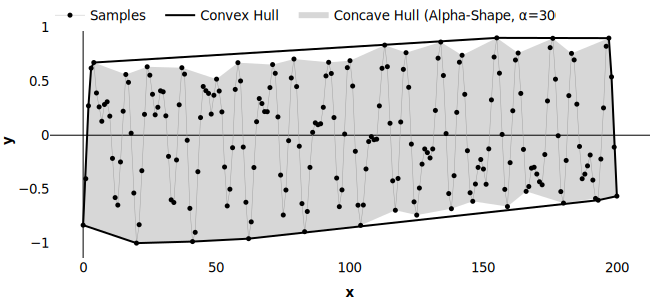
\includegraphics{images/envelope/00ConvexHull.pdf}
  \caption{A discrete signal interpreted as a set of points in the Cartesian plane, and the convex and concave hull at $ \alpha=300 $ defined by it.}
  \label{fig:Hulls}
\end{figure}

The alpha shapes approach is used in areas such as detection of features in images \parencite{2016VarytimidisAlpha}, reconstruction of surfaces from a cloud of points \parencite{2015WuAutomated} and spectroscopy \parencite{2019XuModeling}. 

This last work, which involves the estimation and removal of the Blaze function (a kind of envelope) of an echelle spectrograph, being particularly illustrative of the potential synergy between geometric and DSP approaches.

Other steps in the direction of translating geometric algorithms to the context of envelope detection were made by \textcite{2015YangSkeleton} via an algorithm based on the construction of a skeleton underlying the digital wave of interest, and also via the direct translation of computer vision methods to the task of envelope detection \parencite{2015YangRepresenting}.

Following this path, we present a general approach to envelope detection, exploiting the intrinsic characteristics of a generic, spectrally complex wave, in order to completely avoid the need for manual intervention or parameter tuning.

The rest of this paper is divided as follows: We start by defining as specifically as possible what a temporal envelope is, especially in the context of this work and providing a mathematical definition, in terms of the Hilbert transform, for the case of a narrowband signal.

We proceed to illustrate the representation of a discrete wave used in this work, largely based on the concept of dividing the wave into its constituent pulses, and how it can simplify the algorithm, reducing the high dimensionality generally present in digital representations of waves.

Next, we review methods for the estimation of the curvature of a discrete wave, after which we present our own; this method will then be used to estimate the equivalent circle, that will be used to define the envelope of the wave, via the procedure described in sequence.

In the results section, we present some illustrations of the envelopes obtained with our method, comparing both accuracy and running time with the most common algorithms encountered in the literature. We also suggest an alternative use of the algorithm to identify the negative and positive frontiers of a wave, that can be seen as partial envelopes considering only the positive and negative pulses of a wave, respectively.

We follow with suggestions about how the approach here presented can be useful beyond envelope detection, exemplifying with some applications, such as the extractions of the average waveform of a digital wave, and concluding with commentary on potential future developments of the method.


\subsection{Methods}
After defining what will be considered an envelope in the context of this work, in this section we explore some simplifications that can be applied to a discrete wave, defining the representation that will be used in the subsequent part of the work. 

We next explore the concept of discrete curvature, putting forth our own method, tailored to the definition of the equivalent circle of a wave; we end this section by showing how this circle can be used to identify the envelope of a discrete wave, in a similar approach to that of the alpha shapes theory, but taking advantage of some unique structure present in discrete waves.

\subsubsection{Characterization of a temporal envelope}

The interest in the theory of envelope detection arose in the analog domain, with the widespread adoption of radio communications, where the problem is typically restricted to simple sinusoids, often with well-defined frequencies \parencite{2011TurnerDemodulation}.

In this context, the most mathematically sound definition of an envelope involves the representation of its underlying wave as an analytic signal, as introduced by Gabor in 1946 \parencite{2007HahnHistory}. In his work, \textcite{1946GaborTheory} applies the then relatively new mathematical machinery of the quantum mechanics to unify the time and frequency-domain representations of a wave, showing how the Hilbert transform could be applied to a real signal in order to obtain an equivalent complex signal, later known as the analytic signal.
This analytic signal has the form $ A(t) = S(t) + \mathbb{H}(S(t)) \ \text{i} $ \parencite{2016HePraat} where $ S(t) $ is the original real signal. $ \mathbb{H}(S(t)) $, the Hilbert transform of the original signal, becomes the imaginary part of the analytic signal; the envelope of a signal thus represented can be straightforwardly obtained by the computation of the complex modulus of $ \mathbb{H}(S(t)) $.

Despite its widespread use, and effectiveness in the context of narrowband signals, envelope detection techniques based on the Hilbert transform don't behave well for broadband signals \parencite{2012DauSpeech}, being even physically paradoxical in some cases \parencite{1996Loughlinamplitude}.

Figure \ref{fig:AnalyticSignal} exemplifies the Hilbert envelope, for a pure sinusoid modulated by a polynomial, illustrating the difference in the shape of the envelope in the presence and absence of Gaussian white noise. It is readily noticeable from the figure that, as soon as noise is introduced in the original signal, it is reflected in the envelope.

\begin{figure}[H]
  \centering
    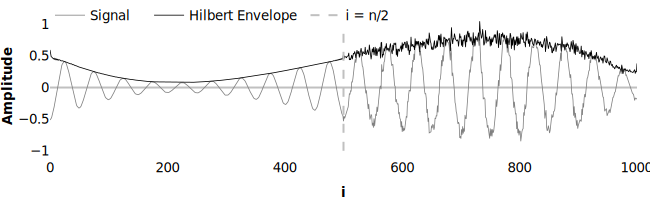
\includegraphics{images/envelope/01AnalyticSignal.pdf}
  \caption{Envelope of a pure sinusoid with a local frequency of 20 cycles modulated by a polynomial of degree 3, as obtained by the Hilbert Transform approach. In the first half, the sinusoid is free of noise, while in the second half Gaussian noise with a standard deviation of $ 1/10 $ of the maximum amplitude of the wave was added to the base signal.}
  \label{fig:AnalyticSignal}
\end{figure}

In general, the problem of envelope detection, or demodulation, can be interpreted as the task of, given a continuous wave $ W(t) $, decomposing it in two components $ E(t) $ and $ C(t) $, such that $ W(t) = E(t) C(t) $ \parencite{2011TurnerDemodulation}. 

$ E(t) $ represents the slow varying part of the wave, also known as the (temporal) envelope, modulator component, or amplitude modulation (AM) of $ W $, while $ C(t) $ models its fast varying part, called throughout the literature as its (temporal) fine structure, carrier component, or frequency modulation (FM).

In the case of broadband signals, the problem of envelope detection of an arbitrary wave is ill-posed, in the sense that an infinite number of pairs of $ E(t) $ and $ C(t) $ can result in the same specific $ W(t) $ \parencite{2011TurnerDemodulation, 2013Mengempirical, 1996Loughlinamplitude}.

We address this problem by assuming $ C(t) $ normalized between $ \{-1, 1\}$. This assumption doesn't cause any loss of generality since, given an arbitrary $ C(t) $, we can obtain its normalization by dividing the function by its absolute global maximum, that is, $ \hat{C}(t) = C(t) / \max(|C(t)|) $, provided that $ \max(|C(t)|) \ne 0 $.

In this work we are concerned with the discrete version of this problem: given a finite digital wave represented by the vector $ \textbf{w} \in \mathbb{R}^n $, instead of the continuous function $ W(t) $, obtaining the temporal envelope of $ \textbf{w} $. 

The preceding definitions can be translated to this discrete scenario assuming that the discrete quantities arise from observing the continuous ones at regular time intervals. In that case, the equality $ i = t \ \text{fps} $ can be used to link both settings, where $ i $ is the index of each observation, $ t $ stands for the time in seconds, and fps is the frame rate, or the number of observations made in the period of a second. We can thus define:

\begin{subequations}\label{eq:Envelope}
\begin{align}
  & \mathbf{w}, \mathbf{e}, \mathbf{c} \in \mathbb{R}^n \\
  & \mathbf{w} = (w_0, w_1, \cdots, w_{n-1}) \\
  & \mathbf{e} = (e_0, e_1, \cdots, e_{n-1}) \\  
  & \mathbf{c} = (c_0, c_1, \cdots, c_{n-1}) \\
  & \mathbf{w} = \mathbf{e} \odot \mathbf{c} \ \therefore \ w_i = e_i c_i \ \forall \ i, \ 0 \le i \le n-1
\end{align}
\end{subequations}

The $ \odot $ operator in \ref{eq:Envelope} stands for the Hadamard product, denoting element-wise multiplication of two vectors. Figure \ref{fig:Envelope} provides an example of the vectors just defined: \textbf{w} is obtained by modulating the normalized carrier wave \textbf{c} using the envelope \textbf{e}.

Note from Figure \ref{fig:Envelope} that, at some local maxima, the envelope is well-defined, being in fact equal to the value of the wave $ w_i $, since $ c_i = 1 $ at those points, rendering $ e_i = 1 w_i $. 

The carrier wave \textbf{c} in the figure is periodic, and normalized between $ \{-1, 1\}$. Each cycle of the wave, then, reaches the value 1 only at its maximum making $ w_i $ equal to the value of the envelope at one point in each cycle.

Image \ref{fig:Envelope}, along with the concave hull illustrated in figure \ref{fig:Hulls}, helps forming the intuition behind the method developed in this work: the idea is to identify the local extrema that touch the envelope, those being also the extrema of each (pseudo-)cycle.

This is accomplished with the use of a circle with a defined radius, large enough to prevent it from reaching the smallest local extrema when "rolled" around the (geometric) representation of the wave. Only the extrema touched by the circle will be marked as part of the envelope.

In the next section, a compatible geometric representation will be formulated, along with the necessary tools to estimate the average curvature of the wave and, consequently, the appropriate radius of the circle.

\begin{figure}[H]
  \centering
    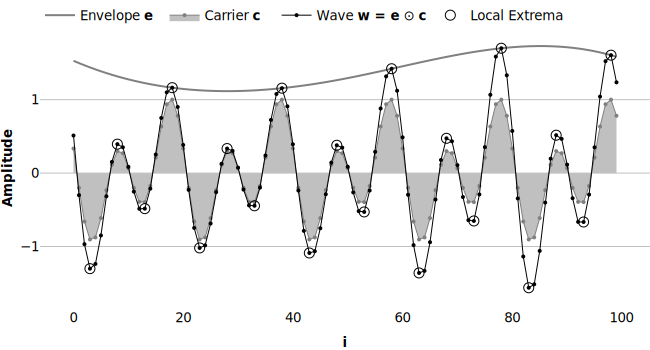
\includegraphics{images/envelope/02Envelope.pdf}
  \caption{Example of a discrete wave \textbf{w} composed by the element-wise multiplication of an envelope \textbf{e} and a carrier \textbf{c}. The local extrema of \textbf{w} are highlighted with a circle.}
  \label{fig:Envelope}
\end{figure}

\subsubsection{Simplified Representation of a Wave}

Instrumental to the method here presented is the definition of a pulse: each time the value of \textbf{w} changes sign, that is, every time the discrete wave \textbf{w} crosses the horizontal axis, the beginning of a pulse is defined, with the next crossing defining its end. This definition is in line with the one presented in \textcite{national1996telecommunications}, where a pulse is defined as a rapid change in the amplitude of a signal, followed by a fast return to the baseline value; zero, in our case.

From \ref{fig:Envelope} and the discussion in the preceding chapter, we can see that only the maximum point of a positive pulse or the minimum point of a negative one can potentially be equal to the envelope and are, thus, our only points of interest. We can then proceed, for the rest of the method, considering only those points, to great computational economy.

For this reason we define P as the set of the points $ \{P_0, P_1, \cdots, P_{m-1}\} $ where $ P_j = (i_j, \lvert w_j \lvert) $, that is, $ \lvert w_j \lvert $, the absolute value of the extrema of each pulse, becomes the ordinate of each point and $ i_j $, its original index, becomes the abscissa.

This relation is illustrated in figure \ref{fig:Pulses}. We call it P to emphasize the connection with the pulses of \textbf{w}.

\begin{figure}[H]
  \centering
    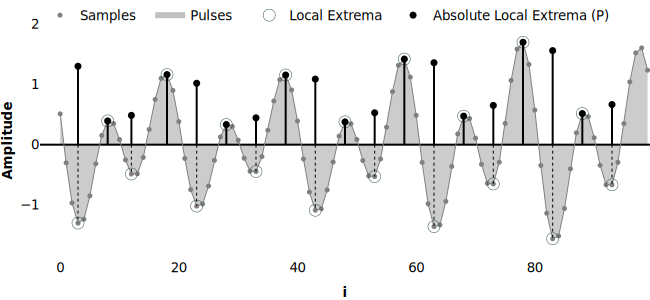
\includegraphics{images/envelope/03Pulses.pdf}
  \caption{Example of a discrete wave \textbf{w} divided into pulses, of which the extrema are highlighted with a circle. P is the set of the points $ P_j = (i_j, \lvert w_j \lvert) $ representing the absolute value of those extrema.}
  \label{fig:Pulses}
\end{figure}

The points in P are not fit for geometric interpretation yet, since the abscissa and ordinate of their orthogonal coordinate system have different units: in the vertical axis, we have a unit related to the instantaneous intensity of the wave, while in the horizontal axis we have the index at which each extremum occurs, ultimately a time-related unit. 

Specifically, this coordinate system has a basis vector $ \mathbf{b} = \{ \mathbf{b}_x, \mathbf{b}_y \}$ with $ \mathbf{b}_x = (a, 0), \mathbf{b}_y = (0, i) $ where $ a $ is an amplitude unit such as decibel, a measure of the instantaneous sound pressure, volt or even a fraction of a fixed maximum value. $ i $ represents the index of the sample, and is linked to time by the aforementioned relation $ i = t \ \text{fps} $.

We are interested in finding a coordinate system where a pulse's amplitude $ \lvert w_j \lvert $ and length would define, on average, a square. 

To achieve that, we divide the basis vector of the original vertical axis by the average of all ordinates, effectively cancelling the unit of the vertical components of the points. We could divide the basis vector of the horizontal axis by the average of the difference between the abscissa of a point and the abscissa of the immediately posterior, likewise eliminating the axis' unit. 

The drawback is that we would lose the direct link between P and \textbf{w} that arises from the fact that the abscissas of the points in P are indices $ i $ of \textbf{w}: we choose instead to leave the abscissa intact and multiply the now unitless vertical basis axis by the average of the difference between the abscissa of a point and the abscissa of the immediately posterior. In this way, both axes will have unit $ i $, and the relationship is preserved, making it easier to recover the envelope points later.

In this new coordinate system we have a basis vector $ \mathbf{b}^\prime = \{ \mathbf{b}^\prime_x, \mathbf{b}^\prime_y \}$ where $ \mathbf{b}^\prime_x = (i, 0) $ and $\mathbf{b}^\prime_y = (0, i) $, related to the original basis vector by equation \ref{eq:Basis}:

\begin{subequations}  \label{eq:Basis}
\begin{align}
\mathbf{b}^\prime_x &= \mathbf{b}_x  \\
\mathbf{b}^\prime_y &= \frac{\left( \frac{i_{m-1} - i_0}{m-1} \right)}{\left( \frac{\sum_{j=0}^{m-1} \lvert w_j \lvert}{m} \right)} \mathbf{b}_y 
\end{align}
\end{subequations}

The effect of this normalization can be seen in the points shown in figure \ref{fig:Vectors}, shown in scale in both coordinate systems. The set V of the vectors from each point of P to the next is also shown in the picture, and it will be used to estimate the average curvature of P. We define this set in equation \ref{eq:Vectors} below.

\begin{equation} \label{eq:Vectors}
\text{V} = \{ v_0, v_1, v_{m-2} \} \quad \text{where} \quad v_k = P_{j+1} - P_j \quad \forall \quad 0 \le k \le m-2
\end{equation}

\begin{figure}[H]
  \centering
    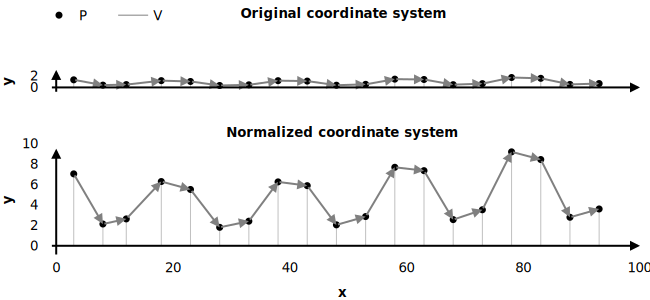
\includegraphics{images/envelope/04Vectors.pdf}
  \caption{The set of points P and the set V of vectors between two adjacent points of P, in both the original and normalized coordinate systems, shown in scale.}
  \label{fig:Vectors}
\end{figure}

\subsubsection{Discrete Curvature Estimation}

Translating the explanation of alpha shapes in \textcite{1994EdelsbrunnerThree} to our context, we can say that the points that are part of the envelope are those touched by a circle of a given radius $ r $, coming from $ y \to \infty $ towards the signal, that is not allowed to contain any point of the signal; Intuitively, one can picture a circle being rolled above the signal, and marking the points it touches as envelope points.

To infer the appropriate radius $ r $ of such circle a measure of discrete curvature is needed. Discrete curvature estimation is an important task in image processing \parencite{2010FleischmannNovel} for which no default definition exists. 

The two possible general approaches are the derivation of direct methods, that use characteristics of the discrete wave to calculate the curvature, or the use of the curvature of a smooth, continuous curve fitted to the discrete wave \parencite{2001CoeurjollyDiscrete}.

Concerning direct methods \textcite{2014CarrollSurvey}, for example, derive three such definitions based on the approximation of a circle by an inscribed, centered and circumscribed polygon. In the context of three-dimensional meshes, \textcite{2016VasaMultivariate} evaluate a range of existing estimators from a multivariate point of view.

Those approaches define the discrete curvature in relation to the vertices of a wave (or mesh, in the three-dimensional case). In our particular case, it wouldn't make sense to talk about the curvature of a single pulse, since it is what our points ultimately represent. Instead, we are interested in the change of direction, what the term curvature ultimately means, between two adjacent pulses, as the vectors in the set V suggests.

We thus proceed to define a discrete curvature measure over the edges of a discrete wave. To that end we are going to apply the definition of smooth curvature as the rate of change of the unit tangent to a curve, noting that this is equivalent to that of the osculating circle \parencite{2016VasaMesh}.


\subsubsection{The Equivalent Circle Approach}

The rationale is to find, for each vector $ v_k \in \text{V} $, the radius $ r_k $ of the equivalent circle whose tangent has the same change in direction, in the same horizontal distance, as the vector of interest, as shown in figure \ref{fig:DiscreteCurvature}. The average curvature of P will then be obtained by the average of all radii $ r_k $.

From figure \ref{fig:DiscreteCurvature} is easy to see that $ r_k = v_{k,x} \sin(\theta_k)$ where $ v_{k,x} $ is the component of $ v_k $ in the horizontal direction; $ \theta_k $ itself can be obtained using the slope $ m_0 = 0 $ of a line in the horizontal direction and the slope $ m_k = v_{k,y} / v_{k,x} $ defined by $ v_k $ via the equality $ \theta_k = \arctan \big( (m_k - m_0) / (1 + m_k m_0) \big) $.

\begin{figure}[H]
  \centering
    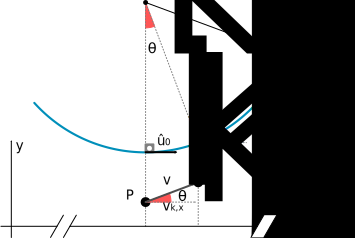
\includegraphics{images/envelope/05DiscreteCurvature.pdf}
  \caption{The tangent unit vector of the circle changes from the horizontal direction in $ \hat{u}_0 $ to an inclination of $ \theta_k $ in $ \hat{u}_1 $, $ \theta_k $ being the angle that the vector $ v_k $ makes with the horizontal direction.}
  \label{fig:DiscreteCurvature}
\end{figure}


The radius of the circle that represents the average curvature of V (and P), and will be used to obtain the envelope of the discrete wave \textbf{w} can be obtained via equation \ref{eq:Radius}:

\begin{equation} \label{eq:Radius}
r = \frac{\sum\limits_{k=0}^{m-2} \left( \frac{v_{k,x} \sqrt{v_{k,x}^2 + v_{k,y}^2}}{ v_{k,y}} \right)}{m-2}
\end{equation}

We need now to construct an algorithm, using the radius just obtained, to identify the points that belong to the envelope. Generally, the algorithm for the alpha shapes approach resorts to the construction of the Delaunay triangulation of the set of points, that is latter filtered to contain only the outer edges. We can adopt a more straightforward method, as our points have a defined structure:

Let $ x_o, y_o \in \mathbb{R}, \quad 0 \le y_o < +\infty $ be the coordinates of the center of a circle with radius $ r $, that can be placed anywhere in the upper plane of the coordinate system;

Let $ P_a, P_b, P_c \in \text{P}, \quad P_a \ne P_b \ne P_c $ be three different points of the set P;

For all circles of center $ x_o, y_o $ and radius $ r $ that can be constructed to pass through any two different points of P, that is, $ \forall \quad P_b, P_c $ such that $ (P_{b,x} - x_o)^2 + (P_{b,y} - y_o)^2 = (P_{c,x} - x_o)^2 + (P_{c,y} - y_o)^2 = r^2 $, $ P_a $ will be part of the set $ E $ of the points belonging to the envelope if and only if none of those circles contain $ P_a $, or $ P_a \in \text{E} \leftrightarrow (P_{b,x} - x_o)^2 + (P_{b,y} - y_o)^2 > r^2 $. Summarizing this, we have equation \ref{eq:InEnvelope}:

\begin{subequations} \label{eq:InEnvelope}
\begin{align}
& P_a \in \text{E} \leftrightarrow (P_{b,x} - x_o)^2 + (P_{b,y} - y_o)^2 > r^2, \\
& \forall \ P_b, P_c \mid (P_{b,x} - x_o)^2 + (P_{b,y} - y_o)^2 = (P_{c,x} - x_o)^2 + (P_{c,y} - y_o)^2 = r^2, \\
& P_a, P_b, P_c \in \text{P}, \quad P_a \ne P_b \ne P_c \quad \text{and} \quad x_o, y_o \in \mathbb{R}, \quad 0 \le y_o < +\infty
\end{align}
\end{subequations}

The algorithm follows directly from the definition in \ref{eq:InEnvelope} after noting that the first and last members of P will always be part of the envelope, since they are reachable by a circle of any radius $ r $. From $ P_0 $, our first pivot point, we construct circles passing through $ P_1, P_2, \cdots, P_d $ until a circle that doesn't contain any point in P is found; $ P_d $ then becomes the new pivot point and is included in E, and this procedure continues until $ P_{m-1} $ is reached.

The procedure is formalized in the algorithm \ref{FindEnvelope}. We don't provide similar algorithmic descriptions of the preceding steps since the Python implementation can easily serve as pseudocode.

\begin{algorithm}[H]
\caption{Retrieve Envelope} \label{FindEnvelope}
\begin{algorithmic}
\STATE \textbf{Given} $ \text{P} = \{P_0, P_1, \cdots, P_{m-1}\}, r $, \textbf{circle}, a function that returns the center of a circle of a given radius passing through two points and \textbf{distance}, a function that returns the Euclidean distance between two points,
\STATE \textbf{Let} $ \text{E} = \{ P_0 \}, \text{id1} = 0, \text{id2} = 1 $
\STATE \textbf{Define} $ P_c = \text{point}, \text{empty} = \text{boolean} $
\WHILE {$ \text{id2} < m $}
  \STATE $ P_c \leftarrow \textbf{circle}(r, P_\text{id1}, P_\text{id2}) $
  \STATE empty $ \leftarrow $ \TRUE 
  \FOR{$ i = \text{id2} + 1 $ \TO $ m $}
    \IF {$ \textbf{distance}(P_c, P_i) < r $}
      \STATE empty $ \leftarrow $ \FALSE
      \STATE id2 $ \leftarrow \text{id2} + 1 $
      \STATE \textbf{break}
    \ENDIF
  \ENDFOR
  \IF {empty}
    \STATE E $ \leftarrow $ E $ \cup \ \{ P_\text{id2} \} $
    \STATE id1 $ \leftarrow $ id2
    \STATE id2 $ \leftarrow \text{id2} + 1 $
  \ENDIF
\ENDWHILE
\end{algorithmic}
\end{algorithm}

The set E obtained via algorithm \ref{FindEnvelope} is a set of points. The most straightforward way to transform those points into the vector $ \textbf{e} \in \mathbb{R}^n $ is via linear interpolation, the approach used in this work. 
It is worth noting, however, that many other procedures are available, both for the interpolation and the smooth approximation of points.

\subsection{Results and Discussion}
Given the lack of a precise definition of what an envelope should be, we begin this section suggesting an empirical metric, based on the behaviour of the carrier wave \textbf{c}. We also comment on some metrics presented in the literature, and compare our algorithm with traditional demodulation approaches, both in relation to execution time and accuracy; to this last end, a numerical indicator is also introduced.

We also illustrate how the method here presented can be used to isolate not only a single envelope of the wave, but the superior and inferior envelopes as well, that we call frontiers, ending the section with a suggestion on how the proposed algorithm can be useful beyond envelope detection, by identifying the approximate locations of the pseudo-cycles in a quasi-periodic wave.

Due to an assortment of factors, such as the unconventional approach presented in this work and the intrinsic difficulty in visualizing discrete waves given their high dimensionality, the authors deemed helpful to provide a companion website with interactive visualizations \parencite{2020TarjanoEnvelope}.

An implementation of the method in pure Python, fully functional, can also be found at the repository dedicated to this work as well as a Python module available at the Python Package Index (PyPI) and conveniently installable via the command `pip install signal-envelope`. Besides, those working under Windows 64-bit can benefit from a specialized dynamic library coded in C++ that is automatically used within this module.


\subsubsection{Quality of an envelope}

There are no agreed-upon objective metrics to assess the quality of an envelope. Recalling figure \ref{fig:Envelope}, however, and the accompanying discussion, an intuitive way is to consider the carrier wave \textbf{c}, and how well it seems to be bounded by the interval $ \{-1, 1\} $. 

To illustrate how the algorithm performs on such metric, we provide the following figures of original discrete waves \textbf{w}, their extracted envelope \textbf{e}, and the inferred carrier, obtained after dividing, element-wise, the original wave by its envelope.

From figure \ref{fig:spoken_voice} it can be seen that the algorithm performs well under the carrier metric. This is especially remarkable for the case of spoken voice, a notorious complex wave with fast changes in pitch and high noise content.

These characteristics are in stark contrast with those of the sang voice in figure \ref{fig:singer_voice}, where a recording of an alto singer is shown; there, the wave is almost periodic, with a stable waveform.

\begin{figure}[H]
  \centering
    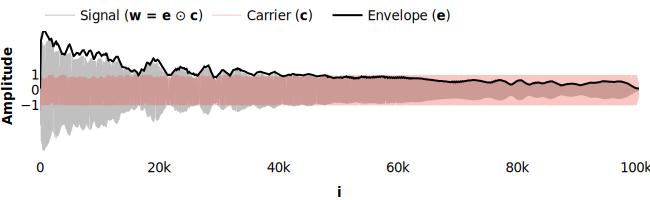
\includegraphics{images/envelope/06Graph_bend.pdf}
  \caption{Signal, envelope and carrier for a record of a bend performed on an electric guitar.}
  \label{fig:Bend}
\end{figure}

\begin{figure}[H]
  \centering
    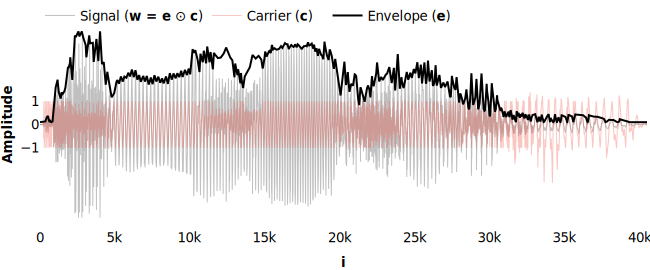
\includegraphics{images/envelope/06Graph_spoken_voice.pdf}
  \caption{Signal, envelope and carrier for a record of male voice uttering the word “amazing”.}
  \label{fig:spoken_voice}
\end{figure}

\begin{figure}[H]
  \centering
    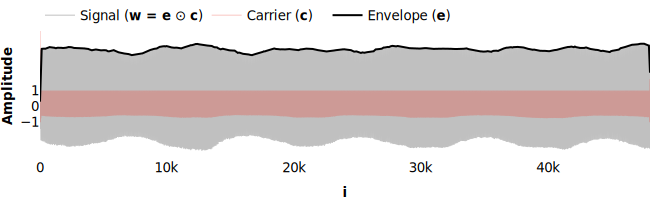
\includegraphics{images/envelope/06Graph_alto.pdf}
  \caption{Signal, envelope and carrier for a record of an alto singer.}
  \label{fig:singer_voice}
\end{figure}

In an effort to formalize the assessment of the quality of temporal envelopes, \textcite{1996Loughlinamplitude} proposed some conditions necessary, but not sufficient, to ensure the physical plausibility of an envelope. We comment briefly below that the algorithm here presented satisfies the four conditions presented.

The first one states that, if a signal is bounded in magnitude, then its envelope should be, as well. Our algorithm complies with this requisite, as the envelope is composed of selected samples from the original signal itself.

The second statement is that if the signal has a finite frequency range, that frequency range must not be exceeded by the envelope. This is only directly applicable in the continuous case, where this condition was proposed.

Nevertheless, if we picture both the wave and the envelope as samples from continuous functions, is easy to see that this is the case for our algorithm; since the envelope is composed by some samples of the digital wave, in the limit where all the samples of the wave are also part of the envelope, we have that the maximum frequency for both is the same. 

In all other cases, the maximum frequency of the envelope will be smaller than that of the original wave. The range of frequencies of the envelope, then, will always lie between zero and the maximum frequency of the original wave.

The third condition states what, for a periodic signal, the envelope should be a straight line with the intercept equal to the amplitude of this signal. Since all the local maxima have the same amplitude in the case of a periodic wave, our envelope will indeed be a straight line, with the same amplitude as the original wave. An example of such behaviour can be observed in figure \ref{fig:Comparison_sinusoid}.

The fourth and last condition states that if a wave is multiplied by a constant, the envelope should also be multiplied by the same constant. That is also the case, again because the points that form the envelope are points of the original wave itself.

\subsubsection{Comparison with traditional algorithms}

Direct comparison with many of the more recent algorithms is made difficult by the unavailability of digital implementations of such works, many designed to process analog signals \parencite[e.g.,][]{2018AssefModeling}.

Nevertheless, insight can be gained from a comparison of the results of the method here proposed with some of the most common envelope extraction algorithms. Specifically, we compare the present method with the following approaches:

\begin{enumerate}
\item Smoothing: This is a relatively simple procedure that, applied to the absolute values of a discrete signal, can provide an approximation of the variation of its amplitude in time. We use the Savitzky-Golay algorithm \parencite{1964SavitzkySmoothing} with a window width of 3001 samples and a cubic polynomial.
\item Filtering: The absolute value of the wave is filtered using a digital implementation of the Butterworth \parencite{butterworth1930theory} low pass filter. We use an order 2 filter with a cut off frequency of 10 Hz.
\item Hilbert Transform: We apply the Hilbert transform to the absolute values of the wave after filtering the original signal with a Butterworth filter with a cut off frequency of 100 Hz, using the absolute value of the analytic signal to obtain the envelope.
\end{enumerate}

In \ref{fig:Comparison_sinusoid} we illustrate the envelope extracted by the conventional algorithms, contrasting it with the result of the method presented in this work, for a simple sinusoid. Note that none of the conventional algorithms complies with the third condition proposed in \textcite{1996Loughlinamplitude} that the envelope of a periodic wave should be a straight line.

\begin{figure}[H]
  \centering
    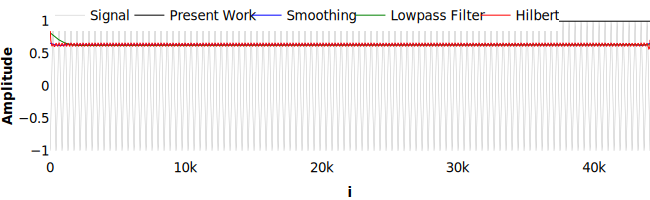
\includegraphics{images/envelope/07Comparison_sinusoid.pdf}
  \caption{Comparison of envelope detection algorithms for a simple sinusoid}
  \label{fig:Comparison_sinusoid}
\end{figure}

For a recording of the key 33 of a grand piano, where parts of the sound are highly percussive and noisy, the Hilbert approach presents considerable oscillations, as can be seen in figure \ref{fig:Comparison_piano}.

\begin{figure}[H]
  \centering
    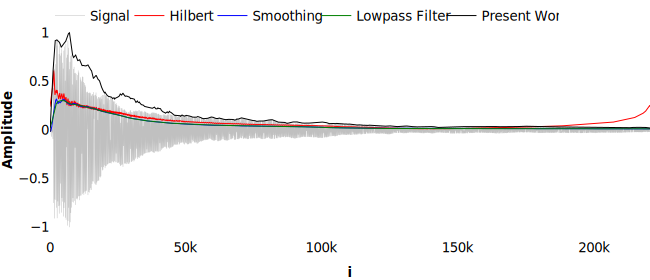
\includegraphics{images/envelope/07Comparison_piano.pdf}
  \caption{Comparison of envelope detection algorithms for the recording of the key 33 of a grand piano}
  \label{fig:Comparison_piano}
\end{figure}

In figure \ref{fig:Comparison_soprano} all envelopes exhibit a similar movement along the samples, but the ones generated by traditional algorithms are undershooting the original wave.

\begin{figure}[H]
  \centering
    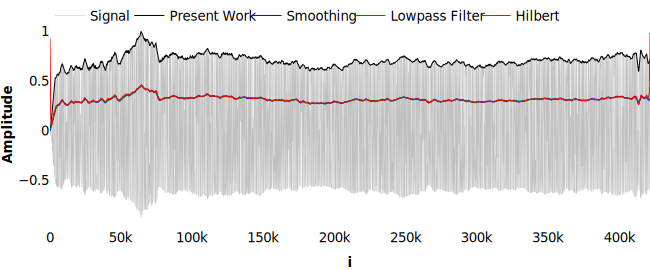
\includegraphics{images/envelope/07Comparison_soprano.pdf}
  \caption{Comparison of envelope detection algorithms for the recording of the vocalization of a soprano singer}
  \label{fig:Comparison_soprano}
\end{figure}


All the traditional methods demanded careful choice of parameters. In the case of the Hilbert transform, pre-processing in the form of filtering was applied. That is in contrast with our method, that organically tunes itself via the automatic choice of the radius of the circle representing the average discrete curvature of the signal.

Table \ref{table:Error_comparison} presents a comparison of the average errors of the techniques. The average error was calculated by the average of the squared distance of the points in the envelope divided by two and the absolute value of the wave. The rationale is that the values of the envelope divided by two should pass near the average of the absolute values of the wave. This metric is only valid for reasonably smooth envelopes, however.

We can see from the table \ref{table:Error_comparison} that the method presented here consistently outperforms the traditional approaches for all waves tested, yielding an error 33\% smaller, on average, than the other methods. It is also worth noting that the errors of the traditional methods are very similar between them.

\begin{table}[H]
\centering
\begin{tabular}{lcccc}
\hline
\multicolumn{5}{c}{\textbf{Average error per frame}} \\
              & Present Work & Smoothing & Low pass & Hilbert \\ 
\hline
alto          & 0.073        & 0.083     & 0.083   & 0.082   \\
bend          & 0.009        & 0.015     & 0.015   & 0.014   \\
piano         & 0.005        & 0.006     & 0.006   & 0.005   \\
brass         & 0.024        & 0.035     & 0.035   & 0.033   \\
soprano       & 0.042        & 0.065     & 0.065   & 0.065   \\
spoken voice  & 0.024        & 0.037     & 0.037   & 0.034   \\
tom           & 0.003        & 0.005     & 0.005   & 0.005   \\
sinusoid      & 0.113        & 0.193     & 0.195   & 0.191   \\ 
\hline
Average       & 0.037        & 0.055     & 0.055   & 0.054  
\end{tabular}
\caption{Comparison of the average errors of the algorithm presented in this work with the most common methods of digital envelope identification. The discrete waves used were normalized between -1 and 1. The average is between the absolute value of those waves and the envelope divided by two.}
\label{table:Error_comparison}
\end{table}

The times taken for the algorithms compared here to process each wave are shown in \ref{table:Time_comparison}. We used specialized implementations available in libraries of the Python programming language. The presented algorithm is in average the second-fastest.

\begin{table}[H]
\centering
\begin{tabular}{lcccc}
\hline
\multicolumn{5}{c}{\textbf{Time in seconds}} \\
              & Present Work & Smoothing & Low pass & Hilbert \\ 
\hline
alto          & 0.008        & 0.101     & 0.007   & 0.011   \\
bend          & 0.030        & 0.226     & 0.012   & 0.131   \\
piano         & 0.034        & 0.374     & 0.014   & 0.042   \\
brass         & 0.032        & 0.297     & 0.011   & 0.045   \\
soprano       & 0.177        & 0.735     & 0.027   & 0.566   \\
spoken voice  & 0.014        & 0.105     & 0.003   & 0.038   \\
tom           & 0.007        & 0.084     & 0.018   & 0.026   \\
sinusoid      & 0.007        & 0.091     & 0.005   & 0.011   \\ 
\hline
Average       & 0.039        & 0.252     & 0.012   & 0.109  
\end{tabular}
\caption{Comparison of the processing time of the algorithm presented in this work with the most common methods of digital envelope identification.}
\label{table:Time_comparison}
\end{table}


\subsubsection{Frontiers}

In practice, is not uncommon for a discrete wave, especially in the case of sound, to present somewhat different positive and negative contours; in those cases, the algorithm here presented can be used independently in the positive and negative pulses of the wave to define two “envelopes”, that we are going to call superior and inferior frontiers.

Figure \ref{fig:FullFrontiers} illustrates the frontiers of six diverse discrete sound waves, as well as an in-detail view of the highlighted segment for each signal. All waves are records of physical sounds, chosen to represent the applicability of the algorithm in real-world scenarios.

\begin{figure}[H]
  \centering
    \includegraphics{images/envelope/08FullFrontiers.pdf}
  \caption{Positive and negative frontiers of six digital waves, as extracted by the algorithm here presented. For each wave, the region highlighted in black is shown in detail besides the whole wave. For each wave, the horizontal axis is the sample number $ i $, while the vertical axis is the normalized amplitude. All 6 waves were recorded at 44100 fps.}
  \label{fig:FullFrontiers}
\end{figure}

The frontiers are satisfactorily detected in the case of harmonic and inharmonic sounds, and are robust in relation to the number of samples and the frequencies of the waves. That is a peculiarity of our algorithm: the traditional algorithms are unable to generate two distinct envelopes for the same wave.


\subsection{Approximated location of pseudo-cycles}

The envelope is shown to add complexity to the spectral representation of a wave \parencite{2019TarjanoNeuro}, and an accurate description of the envelope, while describing the evolution of the instantaneous amplitude of a signal in time, would also simplify further spectral analysis. Figure \ref{fig:Fourier} shows the frequency-domain power spectrum for the wave and the carrier presented in \ref{fig:Envelope}. For the carrier, the power spectrum presents two nonzero values, while the power spectrum for the wave composed of the carrier modulated by the envelope is more complex.

\begin{figure}[H]
  \centering
    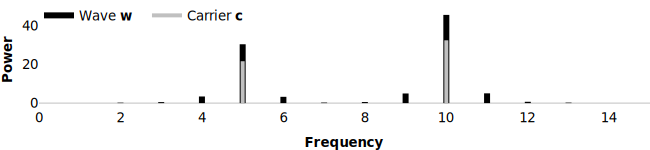
\includegraphics{images/envelope/11Fourier.pdf}
  \caption{Fourier power spectrum for the wave and carrier shown in \ref{fig:Envelope}.}
  \label{fig:Fourier}
\end{figure}

Moreover, the algorithm developed in this work naturally divides a signal into its pseudo-cycles, pinpointing them in the time-domain, thus providing the building blocks for the reconstruction of the fine structure of the wave.

\begin{figure}[H]
  \centering
    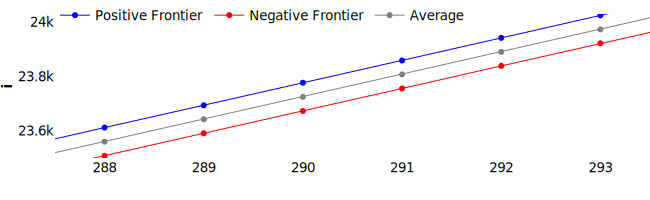
\includegraphics{images/envelope/09PCs.pdf}
  \caption{Section of the lines formed by the positions of the positive and negative frontiers of the digital wave illustrated in \ref{fig:singer_voice}, as extracted by the algorithm presented, and their average.}
  \label{fig:PCs}
\end{figure}

One can see in figure \ref{fig:PCs} a section of the plot of where the local maxima and minima occurs in the recording of an alto singer show in \ref{fig:singer_voice}. The average between the two is also shown. With this information, one can split a discrete wave into its pseudo-cycles, as is illustrated in Figure \ref{fig:AvgPc}: It shows the superposition of this extracted pseudo-cycles, after being normalized by length, and their average. This same average is shown shifted, to exemplify that approximate $C^0$ and $C^1$ continuity is achieved. 

\begin{figure}[H]
  \centering
    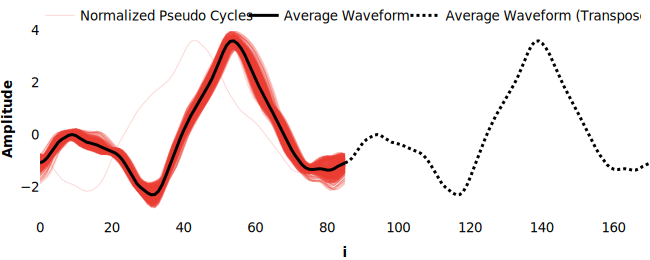
\includegraphics{images/envelope/10AvgPc.pdf}
  \caption{Pseudo-cycles of the wave illustrated in \ref{fig:singer_voice}, segmented and superposed, and their average. The average is also shown shifted by one average period, to illustrate the average continuity.}
  \label{fig:AvgPc}
\end{figure}


\subsection{Conclusion}
This work fills a gap identified in the theory of digital signal processing, where the lack of general procedures for the accurate identification of the temporal envelope of arbitrary waves poses an obstacle to the complete description and eventual manipulation of signals.

By presenting a general approach for envelope detection, and eliminating the need for parameter tuning, we expect to facilitate further research at the many areas that rely on envelope detection techniques, and improve already existing algorithm that have envelope detection as an intermediary step.

Illustrating the efficiency of an algorithm inspired by geometric aspects of a discrete signal on a wide range of real-world signals, we also hope to encourage research in this direction.

The present work also highlights some gaps in our current understanding and definition of temporal envelope and, in so doing, endeavours to motivate further research in this topic, that can ultimately give rise to a more mathematically sound envelope theory, especially concerning broadband waves; suggestions in this direction are also presented.

While relevant in its own accord, the procedure here presented approximately isolates the individual pseudo-cycles of a wave, pinpointing them in the time-domain. 

Similarly, by decomposing a wave into its envelope and carrier, and simplifying the representation of such carrier in the frequency-domain, a rich set of advancements, especially in the areas of sound compression and synthesis in the time and frequency-domains, can be built upon this initial algorithm.

By illustrating how this information can be used to obtain the average waveform of a discrete wave, we hope to encourage research in this area, ultimately leading to alternative representations of discrete waves.


\subsection{Frequency content}


\subsection{Representations} % sound compression paper

% one hot

\section{Pseudo cycles based representation}

Sample-based virtual instruments are the de facto standard for the emulation of real-world acoustic instruments. Nevertheless, little attention is given to the encoding of the samples used in those instruments; lossless formats like WAV or proprietary codecs are common, pushing the on-disk size of those libraries to sizes exceeding the gigabytes. This renders the most realistic digital instruments inaccessible in many but the most high-end hardware; controllers, like electronic drum kits and keyboards and even less robust personal computers are often unable to take advantage of those libraries. We propose a lossy compression algorithm tailored specifically to compress pseudo periodic signals, as those comprising these instruments; due to the highly redundant nature of these sounds, improvements in relation to traditional codecs can be obtained. The algorithm operates entirely in the time domain, avoiding domain conversions common in lossy compression algorithms, thus exhibiting low latency in the decoding phase. It operates iteratively, dividing a signal into its pseudo cycles according to an estimate of the average waveform of those pseudo cycles, which is thus updated, and the process is repeated. We provide C++ source code and implementation of the algorithm, that was used to compare its performance against the MP3, AAC, and Opus codecs, finding the proposed method to be at last 13 times faster in decoding tasks, while maintaining comparable compression rate and quality, as measured by MSE and the ViSQOL library. A website and a GitHub repository with complementary material, where results can be heard, are also available.

Domain specific compression algorithms and codecs exist in many areas. \cite{2016ChenCompressing}, for example, presents a scheme for compressing convolutional neural networks, while \cite{2014CanovasLossy}, besides revising existing methods, proposes two lossy schemes for the compression of quality score data of genomic sequencing. The use of lossy compression for wireless networks of sensors is studied in \cite{2014ZordanPerformance}.

More recently, the work of \cite{2019CalhounExploring} explores the benefits of specific lossy compression algorithms in the context of checkpoints of computational simulations that are stored between simulation sessions; New technologies, such as 3D immersive audio, have propelled specific compression algorithms, such as the one presented in \cite{2021HuAudio}. 

Regarding sample-based digital musical instruments, however, no such specialized algorithms exist despite those signals, being highly uniform, offering a potential for compression that is not present in most general sounds and remains largely unexplored.

This overlook arises in part from the marketing strategy of the majority of those products, where the sheer size of the library is advertised as an equivalent of quality and versatility. An overall prejudice against compressed formats in general from the part of the music production community supports this biased view.

At last some of the criticism directed to the MP3 standard, and lossy codecs in general, is meant to establish a symbolic capital in the face of the crescent struggle between established recording labels and alternative channels of music diffusion, such as streaming services \cite{2020OGradyRethinking}.

The adoption of special compressed formats would enable state-of-the-art digital instruments to be implemented in a wider range of hardware, where the storage costs now make the cost prohibitive, such as electronic drum kits, digital pianos, and even cell phones and tablets, democratizing those tools.

A recent review of the advancements in data compression in general can be found in \cite{2021Jayasankarsurvey}. Accounts of the research in more specific areas, such as video \cite{2019LaudeComprehensive} and image \cite{2014RehmanImage} were also produced recently.

Concerning lossless audio compression, research seems to be lagging when compared to lossy approaches; \cite{2001HansLossless} suggested that a limit was about to be reached at the beginning of the 2000s.

The renaissance of neural networks led to interesting results, for example the use of Generative adversarial networks for audio compression presented in \cite{2018HuangBandwidth}.

The ACER codec, as presented in \cite{2014CunninghamData}, offers an unconventional approach to compression, in that it identifies redundant pieces in a signal that are indexed in a dictionary. The results seem to be satisfactory, from a perceptual standpoint, when compared with MP3 and AAC codecs \cite{2019CunninghamSubjective}.

None of those approaches, however, are designed to take advantage of the redundancies present in harmonic sounds, nor were designed with the low latency requirements imposed by digital musical instruments, especially when operating in real-time; to fill that gap, we propose the method presented in this letter.

\subsection{Methodology} 

A continuous or discrete signal can be interpreted as a succession of consecutive waveforms, each one representing a (pseudo) cycle of the wave. In the case of perfectly periodic signals, those waveforms are identical, and we need only the definition of one waveform to characterize the whole signal. In pseudo periodic waves, on the other hand, there are variations between pseudo cycles, that must be accounted for.

Figure \ref{fig:pseudocycles} illustrates a possible division in pseudo cycles of a segment of the discrete representation of the sound of a bowed cello. It can be seen that the waveform variation between pseudo cycles is very small, on account of the sound being harmonic.

\begin{figure}%[H]
\centerline{\includegraphics[width=\columnwidth]{images/compression/01_pseudocycles.pdf}}
\caption{A discrete wave representing the sound of a bowed cello. The red lines represent the frontiers between successive pseudo cycles, as divided using the presented algorithm.}
\label{fig:pseudocycles}
\end{figure}

This rationale of defining a signal as a series of a modified basis function is presented more formally in \cite{1993SinhaLow}; in that work, however, the bases are wavelets obtained via filter banks applied to the original signal using a pyramid algorithm. A similar approach can be found in \cite{1998SrinivasanHigh}, where a perceptual metric is used. In the presented work this basis is derived directly from the division in pseudo cycles of the underlying signal.

If the wave is sufficiently well-behaved, as is the case with the harmonic sounds used in sample-based digital musical instruments, the bulk of those changes can be attributed to variations in both the amplitude and length of the base waveform; The present algorithm is based on identifying the best basis waveform and registering how it changes over time.

We accomplish that encoding via an iterative algorithm, that divides the signal of interest using a waveform estimate. An updated basis waveform can then be obtained, and the process repeats while improvement in the mean squared error between the initial uncompressed and the compressed signal is being made.

Figure \ref{fig:averagewaveformcello} shows how the base waveform, shown in red, for the cello sample; the base waveform is the average of each individual waveform, after being scaled to the same length. To ensure the continuity of the final wave, the average waveform is rotated between each iteration of the algorithm, so that the absolute vertical distance to zero of its first and last elements is the smallest possible.

\begin{figure}%[H]
\centerline{\includegraphics[width=\columnwidth]{images/compression/02_averagewaveformcello.pdf}}
\caption{The various pseudo cycles in which the signal is divided are shown superimposed, after being scaled to the same length. The average of those individual waveforms is shown in red.}
\label{fig:averagewaveformcello}
\end{figure}

For some signals, the average waveform resembles very closely a sinusoid, as can be seen in Fig. \ref{fig:averagewaveformpiano} that illustrates the average waveform in the case of the sound of a piano key. From a physical perspective, the strings in a piano are excited with an initial impulse left to vibrate undisturbed. After an initial transient period, it is natural that a harmonic mode becomes predominant.

\begin{figure}%[H]
\centerline{\includegraphics[width=\columnwidth]{images/compression/02_averagewaveformpiano.pdf}}
\caption{The various pseudo cycles in which the signal is divided are shown superimposed, after being scaled to the same length. The average of those waveforms is shown in red.}
\label{fig:averagewaveformpiano}
\end{figure}

In figure \ref{fig:periodsenvelope} the envelope and the normalized periods of the wave are shown. Using this data to modulate both the amplitude and the length of the average waveform presented in Fig. \ref{fig:averagewaveformcello} above, one can approximate the original signal, as will be shown in the rest of this chapter.

\begin{figure}%[H]
\centerline{\includegraphics[width=\columnwidth]{images/compression/03_periodsenvelope.pdf}}
\caption{The envelope and the normalized length of each pseudo cycle.}
\label{fig:periodsenvelope}
\end{figure}

While the raw representation of the original cello signal can be viewed as an array with 129867 individual entries, for the compact representation we have 396 pairs of numbers representing the amplitude and length of each pseudo cycle, and the average waveform represented by an array of size 326. The length of the array storing the encoded representation, in the particular case of the cello sample, would be 1118, or approximately 0.86\% of the original, uncompressed representation.

Starting with an initial estimate of the waveform of the signal being processed, one can identify the pseudo cycles of a signal by gradually multiplying, element-wise, different lengths of this estimated waveform with the signal, and observing the highest average value.

For the placement of the initial waveform, one has also to account for the potential phase shift in the signal. This is accomplished by convolving the different lengths of the waveform starting from different positions. For the subsequent placements, the initial position will be already fixed at the end of the preceding pseudo cycle, the length being the only quantity to be estimated.

Figure \ref{fig:tdists} shows how many times a period with a specific length occurs, for 4 different sound samples illustrating different settings. The first two samples are from instruments, a cello, and a piano, and the last two are voices, from a female soprano and a male bass.

The data in blue refers to the initial division of the waves, as obtained by the algorithm presented in \cite{2020TarjanoDigital}. Since the algorithm was primarily designed to identify the envelope of a wave, the variation in the lengths of the pseudo cycles is naturally greater than the red data, where the final result after the application of the current method is shown. 

The distribution of the periods' length tends to present a smaller variance, concentrating around the mode, as the algorithm progresses, and better basis waveforms are found. None of these distributions, as per the Shapiro test, are significantly close to a normal distribution, as can be observed comparing the distributions with the equivalent normal distributions plotted in the figure. 

The normal distributions, as constructed with mean equal to the mode of the periods distribution and standard deviation equal to the standard variation around the mode tend to have a greater spread. Investigating the range between 3 standard deviations around the mode is a very conservative assumption, then, that we can afford to make without compromising the efficiency of the algorithm.

\begin{figure}%[H]
\centerline{\includegraphics[width=\columnwidth]{images/compression/04_Tdist.pdf}}
\caption{Distribution of the number of occurrences of periods lengths for 4 samples, both for the initial waveform in blue and the final waveform in black.}
\label{fig:tdists}
\end{figure}

Fig. \ref{fig:convolution} illustrates, for the cello wave, the procedure for the identification of the first pseudo cycle of the wave, for a particular period. Although only one example is shown in the picture, the various lengths of the waveform are convolved with the beginning of the original signal, and the optimum chosen.

\begin{figure}%[H]
\centerline{\includegraphics[width=\columnwidth]{images/compression/05_convolution.pdf}}
\caption{Identification of the first pseudo cycle. The intensity of the color is proportional to the average of the multiplication between the basis waveform and the underlying original signal. Only one waveform length is shown, translated in intervals of 10 frames.}
\label{fig:convolution}
\end{figure}

For the subsequent periods, the procedure is as illustrated in Fig. \ref{fig:scaling}, as taking the original cello wave as an example: only the length of the basis waveform is changed, using cubic interpolation. At the first iteration, the steps illustrated in both Fig. \ref{fig:convolution} and Fig. \ref{fig:scaling} are performed with the use of a sinusoid, to ensure the best initial division and faster convergence of the algorithm.

\begin{figure}%[H]
\centerline{\includegraphics[width=\columnwidth]{images/compression/06_scaling.pdf}}
\caption{Identification of the second pseudo cycle, by multiplying different lengths of the basis waveform with the underlying original signal. The intensity of the color is proportional to the average of the multiplication.}
\label{fig:scaling}
\end{figure}

\subsection{Results}
In this section, we compare the algorithm here presented with the most common lossy codecs in a variety of sound samples chosen to reflect the proposed immediate application of the algorithm, and thus consist of excerpts from notes from various instruments, as well as singing voice, as would be encountered in the libraries of sample-based instruments. Results can be heard on the website prepared for this letter \cite{2021TarjanoCompression}.

The samples from soprano, mezzo-soprano, and bass singers were obtained by processing sounds from the Vocalset library\cite{2018WilkinsVocalset}, and are licensed under the Creative Commons Attribution 4.0 International. The male singer sample was based on a sample from the Human Voice Dataset \cite{2015Vocoboxvocobox}, available under the MIT License.

The double bass, french horn, flute, and saxophone samples were based on samples freely available at the resources page of the Phillarmonia symphony orchestra website \cite{Philharmonia}, while the piano, cello, and violin samples were processed from the basis samples offered in the University of Iowa Musical Instrument Samples (MIS) \cite{FrittsUniversity}, and are also freely available.

All original samples are uncompressed audio encoded in the WAV format, at a standard frame rate of 44100 fps and a bit rate of 705 kbps, mono that were normalized with long silences manually removed. The format was chosen for its popularity both in general \cite{2014LuoIdentifying} and in sample-based digital instruments.

For the compressed formats, three lossy codecs were chosen. The first format we compare to is the popular MP3, the third layer of the MPEG-1/2 specification, proposed in 1992 \cite{2018BritanakAudio} by the Moving Picture Experts Group. 

The AAC format, in addition to being the formal mp3 successor, is used in services like Apple iTunes and YouTube \cite{2016SeichterAAC}. It was developed by a joint effort between industry representatives such as Dolby and Sony and academic representation through Bell Labs and the University of Hannover, for example \cite{2018BritanakAudio}.

Outside the MPEG committee, the open-source Opus format, standardized by the Internet Engineering Task Force (IETF) in 2012, was chosen. Besides being considered superior to its predecessor Vorbis and the AAC format \cite{2018GunawanPerformance}, the codec supports both speech and music, has very low delay \cite{2013Valinhigh}, being used in real-time audio applications such as WhatsApp \cite{2019SrivastavaSmartphone}.

The Opus codec, along with ACC and MP3, forms the set of the most advanced \cite{2019LaudeComprehensive} and popular \cite{2018KwanObjective} lossy compression formats; Readily available implementations of more experimental algorithms, such as the aforementioned ACER codec \cite{2014CunninghamData}, or the wavelet-based approaches presented in \cite{1993SinhaLow} and \cite{1998SrinivasanHigh} couldn't be found.

All conversions, except for the MP3 encoding done with the Lame library, were made with the FFmpeg library. The PowerShell scripts used are available in the letter's repository \cite{2021TarjanoCompression}. The encoding configurations were chosen in order to generate files with sizes compatible with the present algorithm: for the MP3 format, a bit rate of 8 kb/s and a frame rate of 8000 frames/s was chosen. For the other two formats, no frame rate reduction was needed, and the bit rates were 4 kb/s for the ACC format and 6 kb/s for the Opus format.

As can be seen in the accompanying website, the present work exhibits an average compression rate of 1.09\%, slightly larger than the 0.92\% obtained with the Opus codec, and better than the AAC (1.19\%) and MP3 (1.20\%) codecs.

\subsection{Decoding times}
Encoding times, as can be seen in the accompanying website, are around two times the duration of the original signal, and thus considerably higher than conventional codecs: While part of this discrepancy can be attributed to the immaturity of the implementation when compared to well-established ones, like lame for mp3, with decades of refinement, the majority of the difference can be attributed to the different approach used by the presented algorithm, engaging in a semi exhaustive search for the best basis purely in the time domain.

This approach pays off during the decoding phase, however, since the representation doesn't need to be translated from the frequency domain, for example. In the context of sample-based digital musical instruments, the encoding occurs only once, and takes place in more robust hardware; it is more important to alleviate as much as possible the decoding effort, since, besides enabling the use of more affordable hardware, this task will be performed a far greater number of times.

For digital musical instruments, it is important to maintain latency below 10 milliseconds, since that is the limit above which users start to experiment performance degradation \cite{2002WesselProblems,2016JackEffect}. Table \ref{tab:decoding} compares the absolute decoding times, in milliseconds; it can be seen that the proposed algorithm presents the lowest decoding times, with an average of 12 ms against an average of 163.5 ms of the Opus codec, the second-lowest. Besides, as the reconstruction of the sound is made linearly, pseudo cycle by pseudo cycle, entirely in the time domain, it would be possible to alternate between decoding and reproduction tasks, keeping the latency below the acceptable limit for samples of arbitrary length.

\begin{table}
\centering
\caption{Original Duration and Decoding Times (milliseconds) for the Present Work and the MP3, ACC, and Opus lossy formats.}
\small
\setlength{\tabcolsep}{3pt}
\begin{tabular}{lccccc}
\hline
Sample & Duration & P.W. & MP3 & ACC & Opus \\ 
\hline
cello & 2945 & 11 & 105 & 111 & 136 \\
doublebass & 1388 & 4 & 103 & 201 & 108 \\
flute & 11115 & 17 & 110 & 125 & 117 \\
frenchhorn & 8713 & 21 & 211 & 226 & 223 \\
mezzosoprano & 3259 & 9 & 163 & 147 & 116 \\
piano & 4729 & 19 & 728 & 506 & 520 \\
saxophone & 19825 & 33 & 109 & 115 & 119 \\
singerbass & 2624 & 8 & 123 & 198 & 197 \\
singermale & 1214 & 3 & 104 & 199 & 106 \\
sopranoA & 2598 & 8 & 104 & 120 & 106 \\
sopranoB & 2299 & 5 & 115 & 106 & 106 \\
violin & 2271 & 6 & 111 & 105 & 108 \\ 
% \hline
% Average & 5248.35 & 12.00 & 173.83 & 179.92 & 163.50 \\
% SD & 5486.06 & 8.88 & 177.45 & 111.73 & 118.70 \\
\hline
\end{tabular}
\label{tab:decoding}
\end{table}

\subsection{Quality}

To assess the overall quality of the proposed algorithm, in addition to the computation of the mean square error in relation to the original signal, we made use of the ViSQOL \cite{2020ChinenViSQOL} open-source library developed by Google, designed to substitute subjective listening tests when those are unpractical. According to \cite{2017SloanObjective}, ViSQOL is a more accurate alternative to well-known methods, like PEAQ and POLQA.

Table \ref{tab:quality} shows the ranking of the compressed formats in those metrics: the MP3 codec performed best in all of them; to reach the compatible size with the other codecs, however, it was the only one that needed to be downsampled.

\begin{table}
\centering
\caption{Ranking of the codecs compared under different quality metrics.}
\small
\setlength{\tabcolsep}{3pt}
\begin{tabular}{lcccc}
\hline
Method & Present Work & MP3 & ACC & Opus \\
\hline
MSE & 3 & 1 & 4 & 2 \\
ViSQOL audio & 4 & 1 & 2 & 3 \\
ViSQOL speech & 2 & 1 & 4 & 3 \\
\hline
\end{tabular}
\label{tab:quality}
\end{table}

Although the ViSQOL is designed as a cost-efficient alternative to subjective listening tests, it by any means claims to be a perfect replacement; The reader is strongly encouraged to hear the results in the samples section of the accompanying website  \cite{2021TarjanoCompression}.

Despite performing better than the AAC codec in the objective measures, files compressed with the Opus codec present artifacts, in the majority of the samples, that renders them almost unintelligible. To a lesser extent, that is also the case of the AAC codec.

While presenting an efficient algorithm to compress harmonic signals, with quality on par with the MP3, AAC, and Opus codecs and faster decoding times, immediately applicable to digital musical instruments, this work introduces a new framework for representing pseudo periodic waves, that can serve as a basis for future research. Fig. \ref{fig:waveforms} illustrates this representation, in the case of the cello sample.

Starting from the representation in Fig. \ref{fig:waveforms}, the surface can be approximated by parametric surfaces, or machine learning approaches, providing more robustness in relation to the average waveform approach, for example.

\begin{figure}%[H]
\centerline{\includegraphics[width=1 \columnwidth]{images/compression/07_heatmap.pdf}}
\caption{The evolution of the cello sample waveform over time.}
\label{fig:waveforms}
\end{figure}
  



% \section{References}
\printbibliography %[heading=none]

\newpage
\printglossaries

\end{document}
